\section{Empirical Audit and Numerical Verification}
\label{sec:experiments}

\subsection{Gate G0 Synchronized 5-Minute Market Audit}
\label{sec:exp_audit}

\Cref{tab:g0_audit} reports the Phase~0 Gate~G0 data-routing audit across the synchronized 5-minute \texttt{ohlcv-dev} feed. Both \texttt{VN30F1M} (74,256 bars over 1,516 trading days) and \texttt{VN30INDEX} (50,761 bars over 1,059 trading days), together with all 30 active constituent equities (50 stocks in historical union), achieve $100\%$ completeness across all 10 price, volume, buy-up/sell-down order-flow, and foreign-flow channels.

\begin{table}[t]
  \centering
  \caption{Gate G0 synchronized 5-minute market panel audit across 10 OHLCV, order-flow, and foreign-flow channels.}
  \label{tab:g0_audit}
  \begin{tabular}{lcccc}
    \toprule
    Market Series & 5m Bars & Trading Days & Avg Bars/Day & Coverage (\%) \\
    \midrule
    \texttt{VN30F1M} Futures & 74,256 & 1,516 & 48.98 & 100.0 \\
    \texttt{VN30INDEX} Spot & 50,761 & 1,059 & 47.93 & 100.0 \\
    Active Basket (30 Stocks) & -- & -- & -- & 100.0 \\
    \bottomrule
  \end{tabular}
\end{table}

\subsection{Analytical and Monte Carlo Verification}
\label{sec:exp_math}

We verify every Phase~0 analytical claim numerically. First, exact cost-of-carry affine factorization yields $0.0$ residual under both continuous yields and discrete dividends, while the log-basis upper bound across 10,000 randomized trials exhibits a maximum remainder of $0.640735$ bps. Second, across 12 dyadic refinements ($m = 0, \dots, 11$), the discrete hedging discrepancy decays from $0.03556$ to $1.93 \times 10^{-5}$, attaining a final empirical convergence order of $0.999922$ against the theoretical order of $1.00$ (\Cref{fig:convergence}a).

\begin{figure}[t]
  \centering
  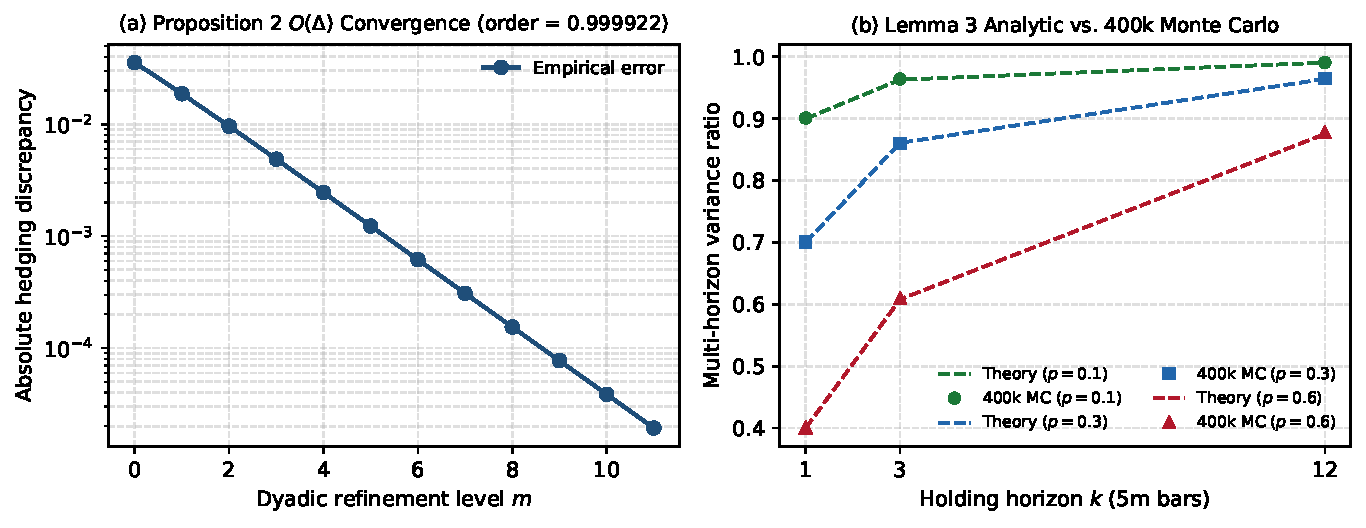
\includegraphics[width=0.98\linewidth]{fig_phase0_convergence.pdf}
  \caption{Empirical verification of Phase 0 analytical bounds: (a) 12-level dyadic refinement confirming first-order $O(\Delta)$ discrete hedging convergence with empirical slope $0.999922$, and (b) 400,000-path Monte Carlo agreement with closed-form multi-horizon variance ratios across $k \in \{1, 3, 12\}$.}
  \label{fig:convergence}
\end{figure}

\begin{table}[t]
  \centering
  \caption{Multi-horizon variance-ratio verification comparing closed-form Lemma 3 values against 400,000 Monte Carlo paths across decay parameter $p$ and holding horizon $k$.}
  \label{tab:lemma3_mc}
  \begin{tabular}{ccccc}
    \toprule
    Decay $p$ & Horizon $k$ & Monte Carlo Ratio & Analytic Ratio & Absolute Error \\
    \midrule
    0.1 & 1 & 0.90107 & 0.90000 & 0.00107 \\
    0.1 & 3 & 0.96420 & 0.96300 & 0.00120 \\
    0.1 & 12 & 0.99077 & 0.99074 & 0.00003 \\
    \midrule
    0.3 & 1 & 0.70086 & 0.70000 & 0.00086 \\
    0.3 & 3 & 0.86012 & 0.86100 & 0.00088 \\
    0.3 & 12 & 0.96464 & 0.96429 & 0.00036 \\
    \midrule
    0.6 & 1 & 0.40019 & 0.40000 & 0.00019 \\
    0.6 & 3 & 0.60927 & 0.60800 & 0.00127 \\
    0.6 & 12 & 0.87739 & 0.87527 & 0.00211 \\
    \bottomrule
  \end{tabular}
\end{table}

Third, \Cref{tab:lemma3_mc} and \Cref{fig:convergence}b confirm close agreement between closed-form multi-horizon variance ratios and 400,000 Monte Carlo trajectories across all 9 $(p, k)$ configurations. Fourth, at stiffness $x = 10^{-13}$, the $\operatorname{expm1}$ transition kernel achieves an absolute error of $1.11 \times 10^{-16}$ compared to $2.44 \times 10^{-4}$ under naive evaluation. Finally, across randomized hypergraph incidences and 10,000 fuzz trials, propagation symmetry holds to $2.78 \times 10^{-17}$, eigenvalues of $\boldsymbol{\Delta}_n$ remain inside $[0.0, 1.0]$, closed-form Gaussian CRPS matches quadrature within $6.51 \times 10^{-19}$, and hard admissibility achieves a $0.00\%$ bound-violation rate.
